\clearpage
\section{Radio Over Fiber Transmission System}

\begin{tcolorbox}	
\begin{tabular}{p{2.75cm} p{0.2cm} p{10.5cm}} 	
\textbf{Student Name}  &:& Celestino Martins\\
\textbf{Starting Date} &:& September 25, 2017\\
\textbf{Goal}          &:& Simulation of Radio over fiber Transmission considering the uplink of base station cooperation systems.
\end{tabular}
\end{tcolorbox}

Radio over fiber (RoF) technology comprises the transmission over fiber technology, where radio signal is modulated onto optical carrier and transmitted over an optical fiber link to provide a simple antenna front ends with increased capacity and broadband wireless services.  In this network a central processing units (CPU) is connected to numerous base stations (BSs) via optic fibers. That means, RoF networks use optic fiber links to distribute radio frequency (RF) signals between the CPU and BSs. The downlink RF signals are distributed from a CPU to many BSs through the fibres, while the uplink signals received at BSs are sent back to the CPU for any signal processing. Figure~\ref{fig_RoFarch} shows a general RoF architecture, where the wireless signals are transported over the optical fiber between a CPU and a set of base stations before being radiated through the air. RoF transmission systems are usually classified into two main categories, depending on the frequency range of the radio signal to be transported: i) RF-over-Fiber; ii) intermediate frequency (IF)-over-Fiber.

\begin{figure}[h!]
    \centering
    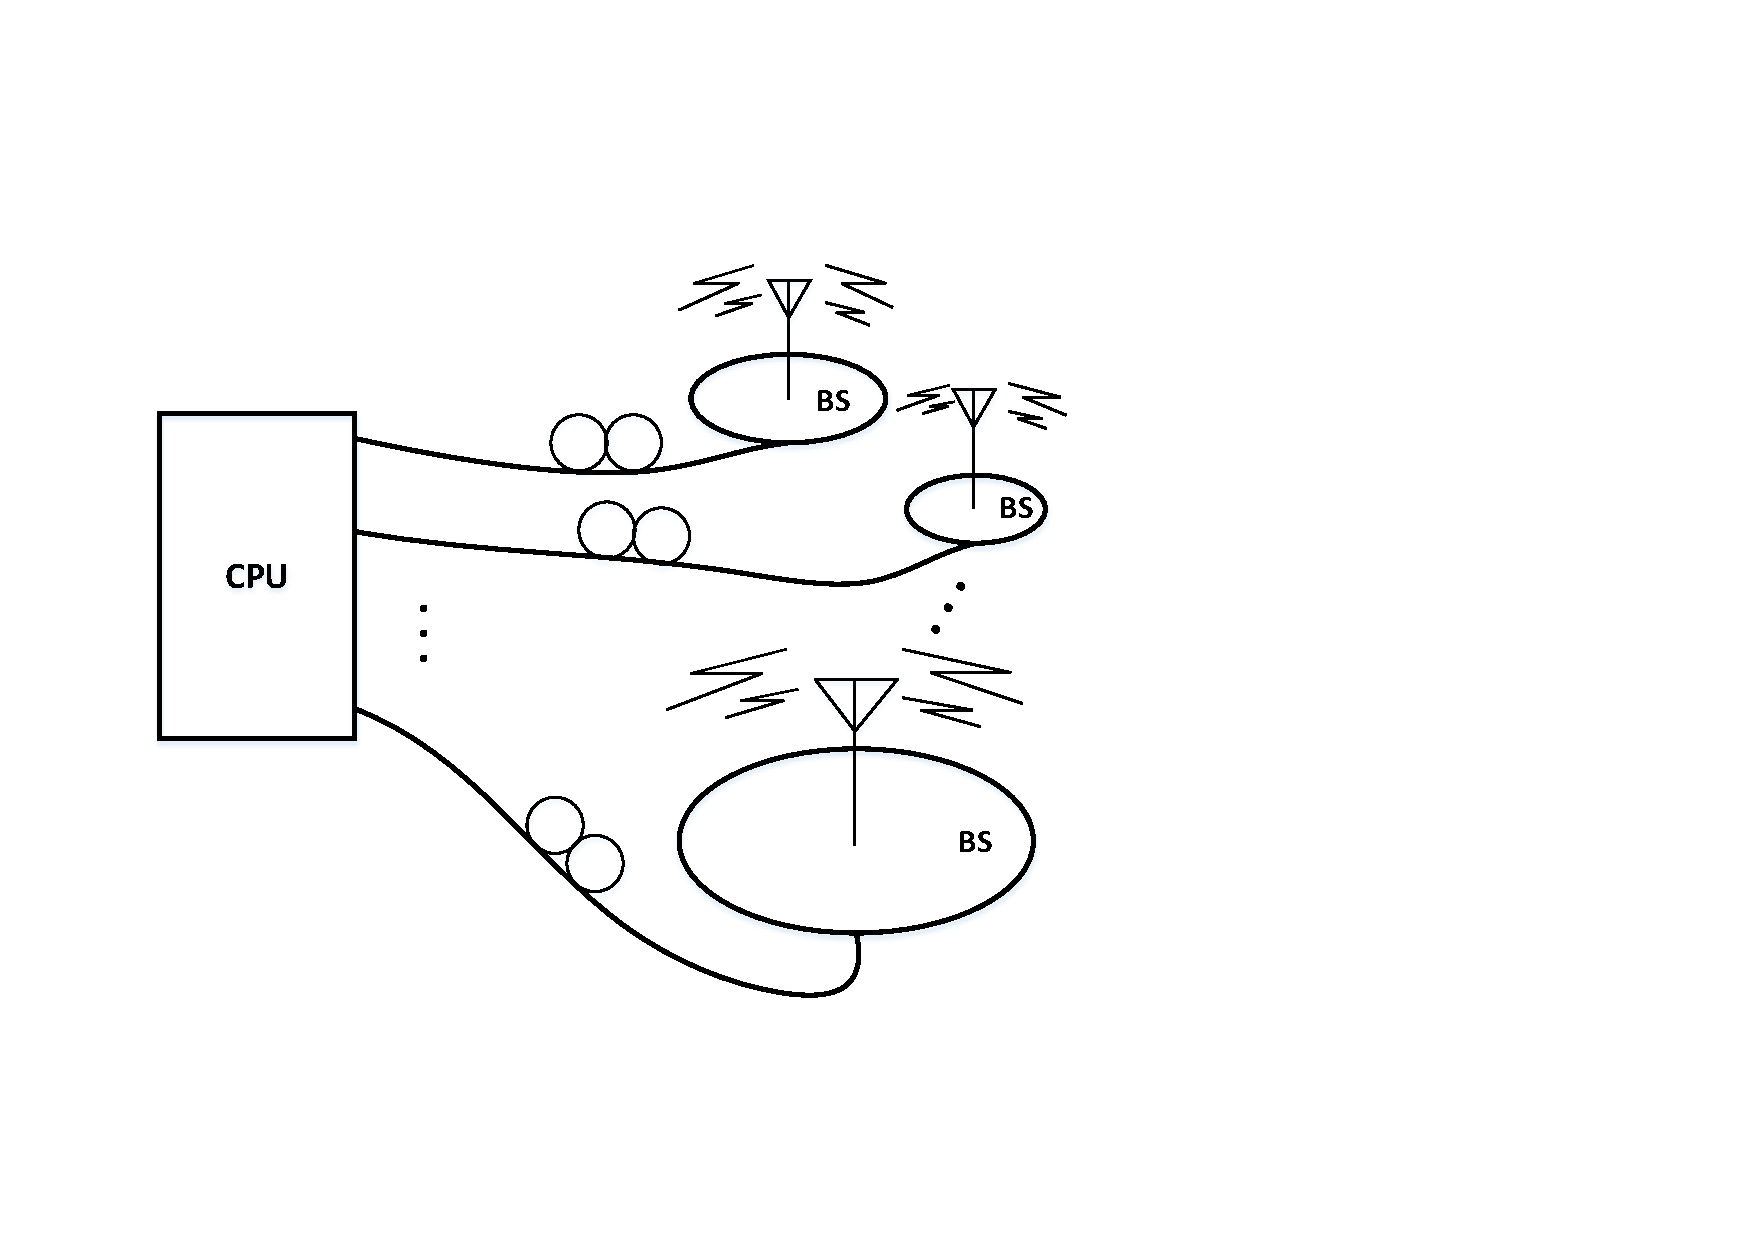
\includegraphics[width=9cm]{./sdf/radio_over_fiber/figures/RoF_architecture.pdf}
    \caption{Schematic showing the concept of a centralized CPU architecture for future integrated optical wireless networks based on RoF.}
    \label{fig_RoFarch}
\end{figure}

\begin{enumerate}[(i)]
\item In RF-over-Fiber architecture, a data-carrying RF (Radio Frequency) signal with a high frequency (usually greater than 10 GHz) is imposed on a lightwave signal before being transported over the optical link. Therefore, wireless signals are optically distributed to base stations directly at high frequencies and converted from the optical to electrical domain at the base stations before being amplified and radiated by an antenna. As a result, no frequency up/down conversion is required at the various base stations, thereby resulting in simple and rather cost-effective implementation is enabled at the base stations.
\item In IF-over-Fiber architecture, an IF (Intermediate Frequency) radio signal with a lower frequency (less than 10 GHz) is used for modulating light before being transported over the optical link. Therefore, before radiation through the air, the signal must be up-converted to RF at the base station.
\end{enumerate}
In addition, the RoF technology can be implemented as analog RoF or digital RoF:
\begin{enumerate}[(i)]
\item In analog RoF technology, the analog signal is transmitted over the optical fiber, being either RF signal, IF signal or baseband BB signal. In the optical transmitter, the RF/IF/BB signal is modulated onto the optical carrier by either using direct or external modulation of the laser. In this case, the signal distribution through RoF has the advantage of simplified BS design, however it is susceptible to fiber chromatic dispersion and nonlinearity generated by optical devices.
\item  In the digitized RoF the wireless carrier RF signal is first digitized prior to transport over the optical link. The digitalization of an RF signal produces a sampled digital signal in a serial form that can be directly modulated on an optical carrier, transmitted over the fiber optic link, and then detected like any other digital information. Modulation of the digital signal onto an optical carrier minimizes the nonlinear effects originating from the optical-to-electrical conversion function presented on analog RoF. In order to use not so high sample rates at the ADC/DAC components generally the bandpass sampling technique i applied to the RF signal.

\end{enumerate}

\subsection{Simulation}
\begin{figure}[h!]
    \centering
    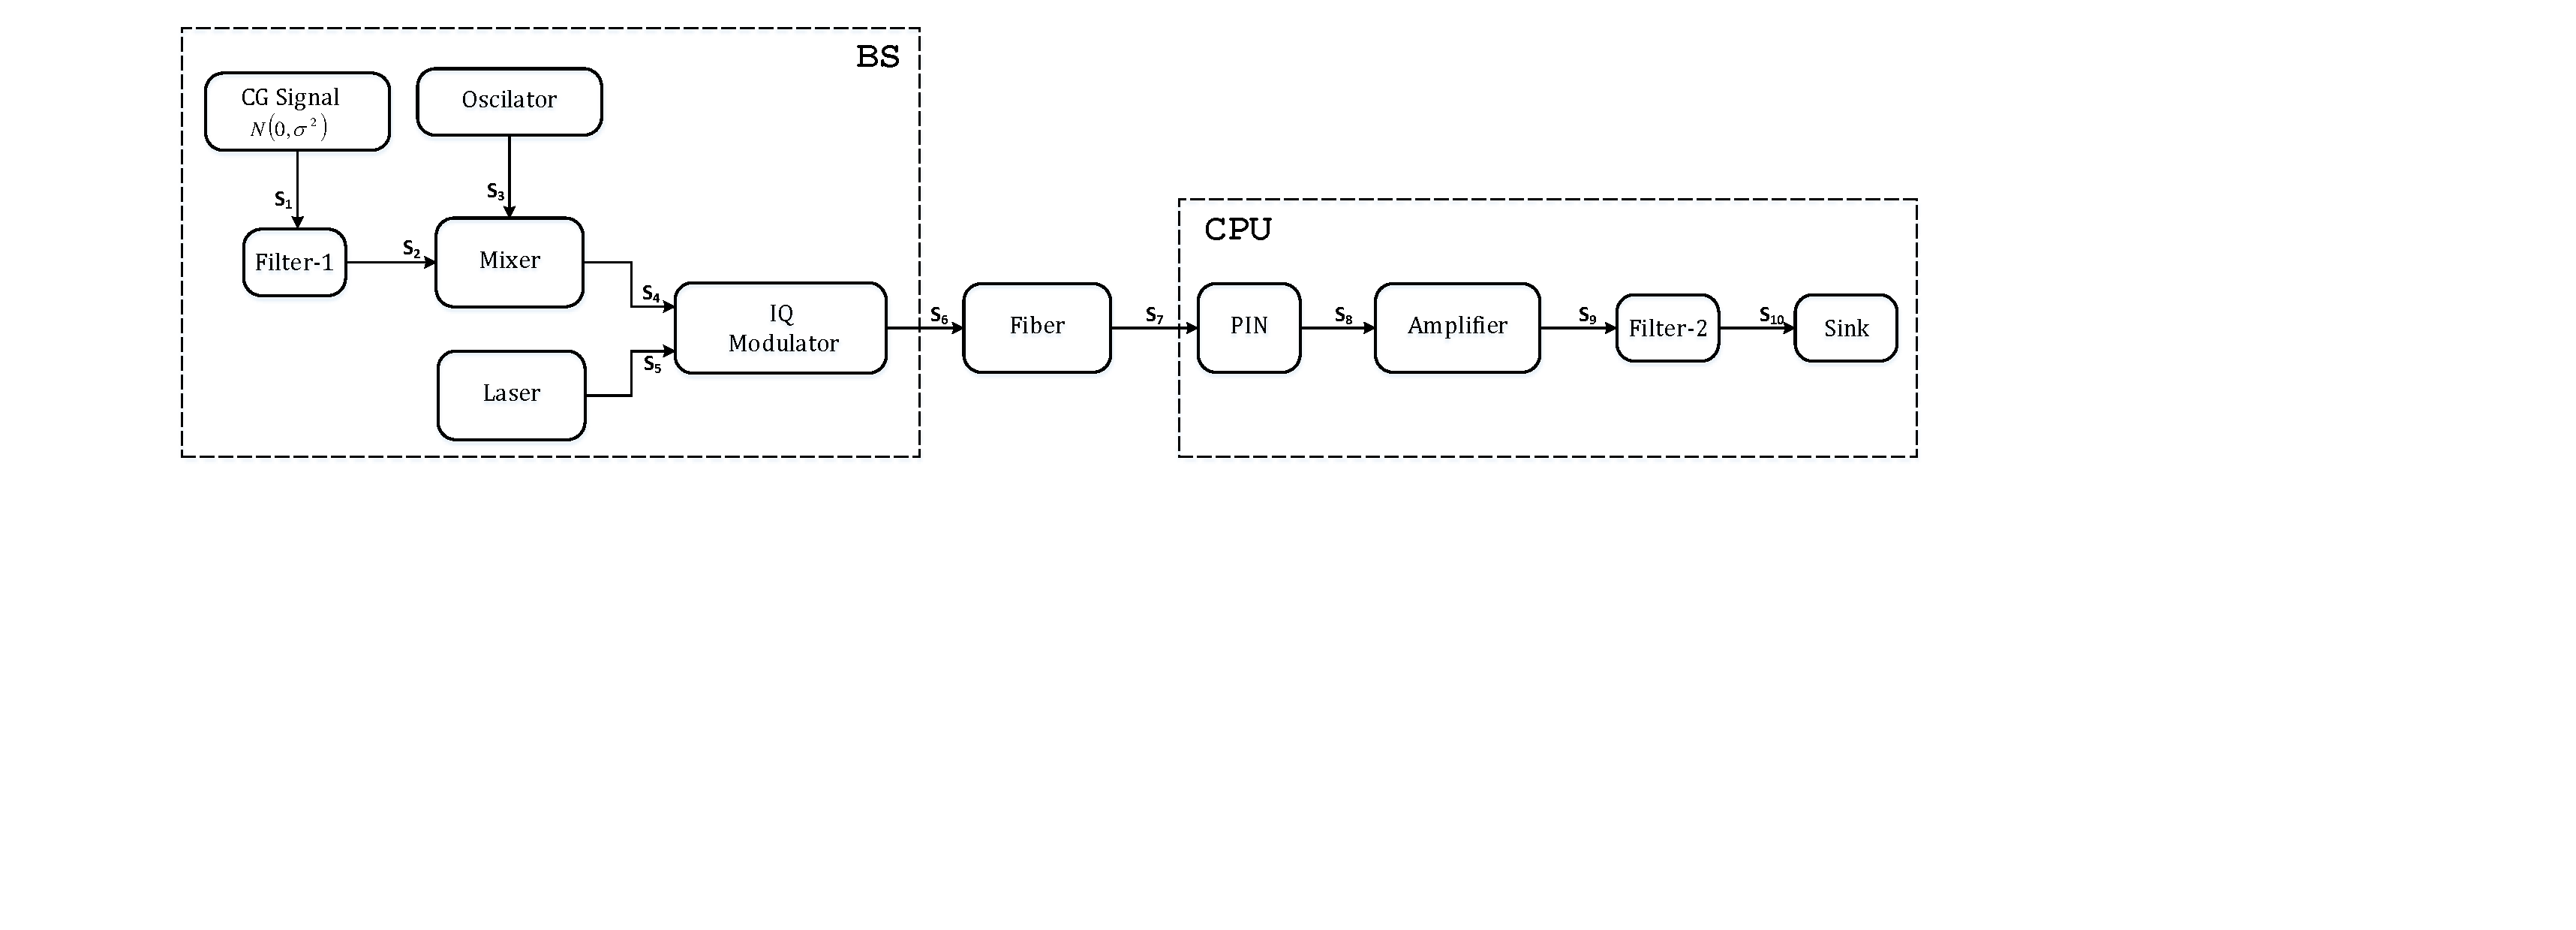
\includegraphics[width=\linewidth]{./sdf/radio_over_fiber/figures/block_diagram_flow.pdf}
    \caption{Simulation setup for the uplink of RoF transmission system. Complex Gaussian (CG); }
    \label{fig_RoFdiagram}
\end{figure}

 Figure~\ref{fig_RoFdiagram} depicts the simulation setup for an uplink of RoF, providing the connection between BS to CPU. At BS, we model the RF signal received from a mobile terminal, as zero mean complex gaussian (CG) signal with a given bandwidth imposed by the low pass filter, Filter-1. The generated baseband signal is then up-converted to RF carrier frequency by utilizing an oscillator and a mixer. In this simulation we consider the RF carrier frequency between 2 to 5 GHz, according to the 5G technologies specifications. The generated RF passband signal modulates optical carrier by utilizing a laser and a mach-zehnder modulator (MZM). The optical signal is then transmitted to CPU using optical fiber. In CPU, the optical signal is detected by a PIN, amplified and followed with an electrical filter. After these operations, digital signal processing techniques can be applied to recover the transmitted signal.

\begin{table*}[h!]
    %\small
    \renewcommand{\arraystretch}{1.3}
    \centering
    \caption{System Input Parameters.}
    \label{system_input_parameters}%
    %\scalebox{0.85}{
    \resizebox{9cm}{!}{
    \begin{tabular}{|c|c|c|}
        \hline
        {$\text{Parameter}$}   & {$\text{Default Value}$}  &  {$\text{Description}$}  \\
        %\cline{2-3}
        \hline
        \hline
        {$\text{sourceMode}$}    & {}      &{}      \\
        \hline
        {$\text{symbolPeriod}$}  & {}    &{}      \\
        \hline
        {$\text{samplePeriod}$}  & {}    &{}      \\
        \hline
        {$\text{numberOfSamplesPerSymbol}$}  & {}    &{}      \\
        \hline
        {$\text{filterType1}$}  & {}    &{}      \\
        \hline
        {$\text{rollOffFactor}$}  & {}    &{}      \\
        \hline
        {$\text{filterType2}$}  & {}    &{}      \\
        \hline
        {$\text{outputOpticalPower}$}  & {}    &{}      \\
        \hline
        {$\text{outputOpticalWavelength}$}  & {}    &{}      \\
        \hline
        {$\text{rfCenterFrequency}$}  & {}    &{}      \\
        \hline
        {$\text{fiberAttenuation}$}  & {}    &{}      \\
        \hline
    \end{tabular}}
\end{table*} 
\begin{table*}[h!]
    \tiny
    \renewcommand{\arraystretch}{1.0}
    \centering
    \caption{Header Files for RoF Transmission System.}
    \label{header_files}%
    %\scalebox{0.85}{
    \resizebox{9cm}{!}{
    \begin{tabular}{|c|c|c|}
        \hline
        {$\text{File Name}$}   & {$\text{Description}$}  &  {$\text{Status}$}  \\
        \hline
        \hline
        {$\text{complex\_gaussian\_signal.h}$}     &{}      &{}      \\
        \hline
        {$\text{pulse\_shaper.h}$}  & {}    &{\checkmark}      \\
        \hline
        {$\text{local\_oscillator.h}$}  & {}    &{\checkmark}      \\
        \hline
        {$\text{mixer.h}$}  & {}    &{}      \\
        \hline
        {$\text{cw\_laser.h}$}  & {}    &{}      \\
        \hline
        {$\text{iq\_modulator.h}$}  & {}    &{\checkmark}      \\
        \hline
        {$\text{fiber.h}$}  & {}    &{}      \\
        \hline
        {$\text{pin.h}$}  & {}    &{}      \\
        \hline
        {$\text{amplifier.h}$}  & {}    &{}      \\
        \hline
        {$\text{filter\_rx.h}$}  & {}    &{}      \\
        \hline
        {$\text{sink.h}$}  & {}    &{\checkmark}      \\
        \hline
        {$\text{netxpto.h}$}  & {}    &{\checkmark}      \\
        \hline
    \end{tabular}}
\end{table*} 
\begin{table*}[h!]
    \tiny
    \renewcommand{\arraystretch}{1.0}
    \centering
    \caption{Source Files for RoF Transmission System.}
    \label{source_files}%
    %\scalebox{0.85}{
    \resizebox{9cm}{!}{
    \begin{tabular}{|c|c|c|}
        \hline
        {$\text{File Name}$}   & {$\text{Description}$}  &  {$\text{Status}$}  \\
        \hline
        \hline
        {$\text{complex\_gaussian\_signal.cpp}$}     &{}      &{}      \\
        \hline
        {$\text{pulse\_shaper.cpp}$}  & {}    &{\checkmark}      \\
        \hline
        {$\text{local\_oscillator.cpp}$}  & {}    &{\checkmark}      \\
        \hline
        {$\text{mixer.cpp}$}  & {}    &{}      \\
        \hline
        {$\text{cw\_laser.cpp}$}  & {}    &{}      \\
        \hline
        {$\text{iq\_modulator.cpp}$}  & {}    &{\checkmark}      \\
        \hline
        {$\text{fiber.cpp}$}  & {}    &{}      \\
        \hline
        {$\text{pin.cpp}$}  & {}    &{}      \\
        \hline
        {$\text{amplifier.cpp}$}  & {}    &{}      \\
        \hline
        {$\text{filter\_rx.cpp}$}  & {}    &{}      \\
        \hline
        {$\text{sink.cpp}$}  & {}    &{\checkmark}      \\
        \hline
        {$\text{netxpto.cpp}$}  & {}    &{\checkmark}      \\
        \hline
    \end{tabular}}
\end{table*} 
\subsection{Experimental}
